%==========================================================================
%Template File for Evolutionary Computation Symposium
%==========================================================================
\documentclass[a4paper,11pt,twocolumn]{jarticle}
\usepackage{evocomp}
\usepackage{fancyhdr}
\usepackage[linesnumbered,ruled]{algorithm2e}
\usepackage{graphicx}
\usepackage{subcaption}
\usepackage[table,dvipsnames]{xcolor}% http://ctan.org/pkg/xcolor

% Declares special characters to be used in equations:
\newcommand{\B}{{\mathbb{B}}}
\newcommand{\I}{{\mathbb{I}}}
\newcommand{\E}{{\mathbb{E}}}
\newcommand{\R}{{\mathbb{R}}}
\newcommand{\Rnn}{{\mathbb{R}_+}}           % { x ∈ R ∣ x ≥ 0 }
\newcommand{\Rp}{{\mathbb{R}_+^*}}          % { x ∈ R ∣ x > 0 }
\newcommand{\N}{{\mathbb{N}}}
\newcommand{\Np}{{\mathbb{N}_+^*}}          % { x ∈ N ∣ x > 0 }

\pagestyle{empty}

\renewcommand{\headrulewidth}{0.0pt}
\renewcommand{\footrulewidth}{0.0pt}

\renewcommand\refname{References}

\begin{document}
\twocolumn[%
\begin{center}

\beginheader

\jtitle%
{An Evolutionary-Computing Based Framework for Solving Simultaneous Continuous Games}

\begin{authors}
\name{1}{Rui Leite},
\name{1}{Hernan Aguirre},
\name{1}{Kiyoshi Tanaka},
\end{authors}



\begin{affiliation}
\aff{1}{Graduate School of Medicine, Science and Technology, Shinshu University},
\end{affiliation}

\endheader

\end{center}
]

\etitle{An Evolutionary-Computing Based Framework for Solving Simultaneous Continuous Games}

\ename{1}{Rui Leite(23hs201j@shinshu-u.ac.jp)}
\ename{1}{Hernan Aguirre(ahernan@shinshu-u.ac.jp)}
\ename{1}{Kiyoshi Tanaka(ktanaka@shinshu-u.ac.jp)}

\eaff{1}{%
Graduate School of Medicine, Science and Technology, Shinshu University
}

\vspace{3mm}

\kanjiskip=.1zw plus 3pt minus 3pt
\xkanjiskip=.1zw plus 3pt minus 3pt

\section{Introduction}

In modern cybersecurity contexts, situations such as Advanced Persistent Threats (APT) have highlighted the limitations of traditional defense mechanisms, underscoring the need for proactive strategies that assume eventual breaches.
Game-theoretical models are developed in this domain with the goal of deriving policy best practices from the so called ``game solutions''.
In particular, FlipIt \cite{dijk2013flipit} is one such model, simulating stealthy takeovers of a resource being contested by two adversarial agents: a defender and an attacker.

Players have objectives, which are usually conflicting.
The goal of the analyst is to find the so called Nash Equilibria (NE) of the game \cite{bonanno2018game}, which are states where all players successfully maximize their payoffs given the strategies of the other players.
This is not equivalent to treating a game model as a Multi-Objective Optimization Problem (MOOP), as the players are not cooperating towards a common global optimal, but rather are more prone to sabotage each other's efforts.

Recent extensions of FlipIt incorporate multi-objective and continuous strategy spaces, enabling more complex models that better reflect real-world cyber scenarios.
For instance, our previous approach \cite{leite2024cec} introduced infrastructure enhancements, which model the benefits of passive defenses like firewalls.
However, such extensions increasingly complicate the determination of NE to the point where analytical and even existing numerical methods become impractical.
This is why we also explored the use of Co-Evolutionary Algorithms (CoEA) for estimating solutions.
To the best of our knowledge, until the present work, no other numerical method has been demonstrated for solving continuous games of simultaneous decision with multi-objective players and an infinite number of solutions.
On the other hand, while effective, this approach presented challenges in terms of architectural complexity and noisy estimations.

In this paper, we present a novel evolutionary-computing based optimization procedure for continuous games of simultaneous decision, specifically aimed at providing a more comprehensive framework for approximating game solutions even when the objective space is continuous and may therefore potentially contain an infinite number of game solutions.
The proposed method shall appear intuitive to researchers in Game Theory, because it generalizes the basic analytical methods, but also to researchers in Computational Optimization, because it leverages concepts of this field to transform an otherwise infinite problem into a finite set of optimization ones.
Through experimental validation, we demonstrate the method's convergence to a finite but representative number of game solutions, with noise being expected to decrease as more computing resources are allocated.

Beyond the concrete basic algorithmic implementation demonstrated in this work, the proposed method contributes a general abstract procedure, which we hope will guide the development of new, more efficient methods for solving game theory models involving simultaneous decision, continuous decision spaces, and any number of players and solutions, with applications beyond FlipIt.

The remainder of this paper is organized as follows: Section \ref{relatedworks} reviews related work; Section \ref{algorithm} describes the proposed abstract and concrete procedures; Section \ref{methodology} presents the experimental setup; Section \ref{results} discusses our findings; and Section \ref{conclusions} concludes with potential avenues for future research.


\section{Related Work}
\label{relatedworks}


\subsection{Game Theory and Nash Equilibria}
\label{gametheory}

Games with simultaneous decision by all players can be modeled by a quadruple $\left (I, (S_0, S_1, \dots, S_{n-1}), O, f \right )$ \cite{bonanno2018game}, comprised of a list of player identifiers $I = \{0, 1, \dots, n-1\}$ (where $n \geq 2$ is the number of players), a list containing one strategy set $S_p$ per player $p \in I$, a set $O$ of possible outcomes, and a payoff function $f$.
Each strategy set $S_p$ contains all possible strategies that player $p$ may choose; if the player controls multiple variables simultaneously, the strategy set would be the Cartesian product of their corresponding sets (i.e., for a boolean and an integer, $S_p = \{0, 1\} \times \I$).
In Game Theory, a strategy profile is a tuple of game decisions, one or more for each player, that defines a complete game scenario.
Any strategy profile is, thus, $s \in S$ such that $S = S_0 \times S_1 \times \dots \times S_{n-1}$.
We can think of a strategy profile as the input vector for a game evaluation, which is performed by $f: S \rightarrow O$ and outputs the payoff vector ($o \in O$) containing game results for all players.

As an example, let us consider a famous discrete, single-objective game of simultaneous decision called the Prisoner's Dilemma \cite{tucker1983mathematics}, where each of two prisoners (the players) can choose between remaining silent or betraying the other prisoner (their accomplice) by confessing their crime.
Their sole objective is to minimize their own sentence.
The authorities have enough evidence to convict both prisoners of a minor crime, but they need a confession to convict them of a major crime, so they offer each player (separately) the following deal: if the prisoner confesses, they will be released as long as the other player remains silent, while the latter will be convicted of the major crime.
If both confess, they will both be convicted of the major crime, though with a slightly reduced sentence for cooperating.
If both remain silent, they will both be convicted of the minor crime.
We can model this game as shown in Table \ref{tab:prisonersdilemma}, with each player trying to maximize their payoff.
Both players are aware of the payoffs and make their decisions simultaneously (i.e., they do not know each other's decision until both decisions have been made).

\begin{table}[h]
\centering
\begin{tabular}{|c|c|c|}
\hline
\textbf{Strategy profile} & \textbf{Payoff vector} \\
\hline
Silent,  Silent  & -1, -1 \\
Silent,  Confess & -9,  0 \\
Confess, Silent  &  0, -9 \\
Confess, Confess & -5, -5 \\
\hline
\end{tabular}
\caption{Strategy profiles and their payoffs for the Prisoner's Dilemma.}
\label{tab:prisonersdilemma}
\end{table}


The procedure for ``solving'' such games is to find the NE \cite{bonanno2018game}, whose basic form is the Pure-Strategy Nash Equilibria (PSNE), defined here as a subset $E$ from $S$, and comprised of each strategy profile $s^* = (s^*_0, s^*_1, \dots, s^*_{n-1})$ such that:

\begin{equation}
    \forall{p} \forall{s_p}~ f(s^*) \succeq_p f(s^*_0, \dots, s^*_{p-1}, s_p, s^*_{p+1}, \dots, s^*_{n-1})
\end{equation}

Here, all $s_i \in S_i$ and all $s^*_j \in S_j$, and $\succeq_p$ is a relation such that $a \succeq_p b$ denotes that $p$'s perceived outcome from $a$ is preferred to that of $b$ ($a, b \in O$).

There are many interpretations \cite{bonanno2018game} for an NE state $s^* \in E$, one of them being that in it, no player has an incentive to unilaterally change their decision.
Another common interpretation is that in it all players are playing a best response to the decisions of the other players simultaneously (i.e., each is playing a ``best response to the best responses'').
One should also note that, in a NE, no player regrets their choice even after knowing the decisions of the other players (given that all of them chose their strategy for that NE and are therefore playing a best response).
For all of these reasons, such equilibria are often seen as ``solutions'' to a game model, because they reflect the choices that rational players would make, as long as they are aware of the game dynamics and given that the model correctly incorporates players' preferences.

For finite games, as is the case of the Prisoner's Dilemma, the PSNE can be easily found analytically.
The classic procedure can be summarized as follows.
First, a payoff matrix like Table \ref{tab:payoffmatrix} is created with dimensions given by the sizes of the strategy sets.
The payoff vectors are then filled in for each strategy profile.
Next, for each player, we mark their preferred payoff for each unique combination of choices by their opponents.
In the example, the best responses for prisoners 1 and 2 are highlighted in blue and red, respectively.
The PSNE are identified at the end of this process as the strategy profiles for which all players get their preferred payoff simultaneously (i.e., player are all playing a best response against each other).

\begin{table}[h]
    \centering
    \begin{tabular}{|c|c|c|}
        \hline
        & \textbf{Silent} & \textbf{Confess} \\
        \hline
        \textbf{Silent} & -1, -1 & -9, \colorbox{Red!25}{0} \\
        \hline
        \textbf{Confess} & \colorbox{Cyan!25}{0}, -9 & \cellcolor{LimeGreen!50}{
            \colorbox{Cyan!25}{-5}, \colorbox{Red!25}{-5}
        } \\
        \hline
    \end{tabular}
    \caption{Payoff matrix for the Prisoner's Dilemma; the only Nash Equilibrium is highlighted in green.}
    \label{tab:payoffmatrix}
\end{table}



\subsection{FlipIt and its Extensions}

The problem with this procedure is that it is not feasible for continuous games, as the number of possible strategy profiles is infinite.
This is the case for FlipIt \cite{dijk2013flipit} and its extensions \cite{laszka2014flipthem} \cite{sherfield2018flipthem}.

In the original FlipIt game, two players ($I = \left\{ 0, 1 \right\}$) compete for control of a resource.
The resource is an abstraction for a computational resource which the defender player wishes to protect, such as a computer, a network or a password.
The attacker player, on the other hand, wishes to compromise the resource.
Only one player can control the resource at any given time; the players can make moves at any point along a continuous timeline to seize control of it.
The more time a player spends in control of the resource, the higher their payoff (represented here as $\beta_i$ where $i=0$ denotes the defender and $i=1$ the attacker).
Each move incurs a cost ($k_i$) that negatively impacts player $i$'s $\beta_i$.

The manner in which FlipIt is commonly solved involves defining a set of strategy classes from which the players can choose, and which in turn determine the players' move times.
Such classes are also often parameterized, allowing for finer control over the exact move times.
The strategy class we will focus on is the Periodic Strategy (PS), where the players move at regular intervals.
PS is fully characterized by a scalar move rate $\alpha$, which determines the time between moves by the adopting player.
As a consequence, a PS game of FlipIt can be modeled as a quadruple $\left (I=\left\{ 0,1 \right\}, (S_0=\Rnn, S_1=\Rnn), O=\R \times \R, f \right )$ \footnote{We use $\R$ to denote the set of real numbers, and $\Rnn$ for the set of non-negative real numbers.}.
The strategy sets represent each player's choices for $\alpha$, and the fact that they are infinite means that the simple, classic procedure presented in Subsection \ref{gametheory} not applicable.
The best responses for this game could, instead, be successfully determined algebraically \cite{dijk2013flipit}, resulting in analytical expressions for $f$ and the $E$; however, the same is not true for more complex strategies for FlipIt, and/or for some of its extensions, and/or for scenarios where the opponents can choose from many different classes of strategies.

Is this paper, we consider the FlipIt with Infrastructure Enhancement (IE) \cite{leite2024cec}, an extension of FlipIt where the defender can use IE to increase the resource's resilience to attacks.
The main idea is that, for PS games of FlipIt with IE, the defender's strategy set becomes $S_0=\Rnn \times \Rnn$ to accommodate a new decision variable, $\phi$ (the amount of IE), which impacts the resource resilience to attacks, but also incurs in a one-time cost of $c\phi$ monetary units, where $c$ is a game parameter much like $k_0$ and $k_1$ mentioned earlier.
The objective space is now $O = \R \times \R \times \R$, with an additional component accounting for the defender's new objective, maximizing $K(\phi) = -c\phi$ (i.e., minimizing monetary costs).
Analytical expressions are determined for this case \cite{leite2024cec}, which provide us with an opportunity to validate our proposed method.
The ideal PSNE curve and its resulting outcomes are shown in Fig.~\ref{fig:analytical_decision_space} and Fig.~\ref{fig:analytical_objective_space}, respectively.

\begin{figure}[h]
    \centering
    % Converted with: pdftops -eps figs/analytical_curve_decision_space.pdf
    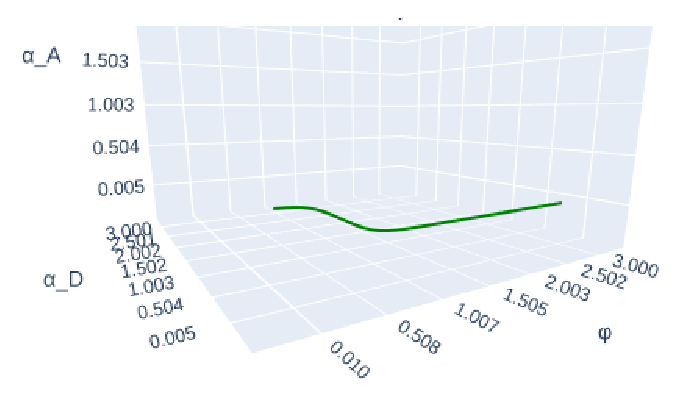
\includegraphics[width=0.9\linewidth]{figs/analytical_curve_decision_space.eps}
    \caption{Analytical PSNE curve for FlipIt with IE.}
    \label{fig:analytical_decision_space}
\end{figure}

\begin{figure}[h]
    \centering
    % Converted with: pdftops -eps figs/analytical_curve_objective_space.pdf
    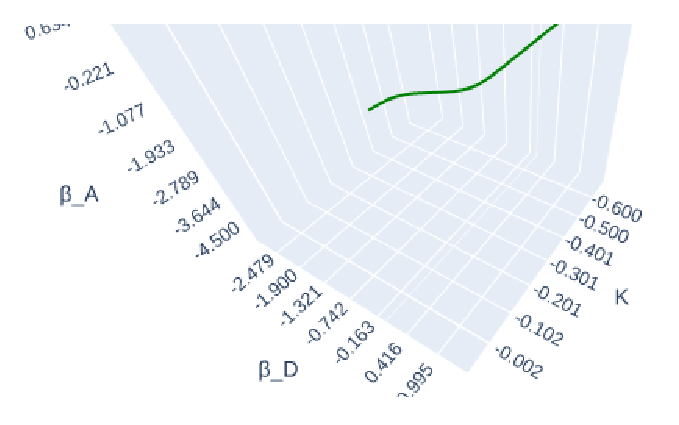
\includegraphics[width=0.9\linewidth]{figs/analytical_curve_objective_space.eps}
    \caption{Payoff for the PSNE curve.}
    \label{fig:analytical_objective_space}
\end{figure}

A computational approach leveraging CoEAs was first proposed by \cite{sherfield2018flipthem}.
His method leverages one population of defender strategies and one population of attacker strategies, which are co-evolved to find a PSNE.
However, it could not be immediately generalized to multi-objective players, especially when the number of solutions is infinite.
Other authors presented a method for solving continuous games of simultaneous decision which could, theoretically, be generalized to accommodate multi-objective players, and was tailored to find many solutions \cite{lung2008computing} \cite{lung2020pareto}; however, in our tests with FlipIt with IE, it only converged to one equilibrium.
This method also uses concepts that are not familiar to researchers in Game Theory or Computational Optimization, which may hinder its adoption by the community.


\section{Proposed Approach}
\label{algorithm}

The proposed approach aims to solve continuous games of simultaneous decision, where each player seeks to maximize their payoff (greedy players).
It is important to note that we present both a general abstract framework (idealized procedure) and a concrete implementation (approximation procedure) for numerically solving such games.
While largely inspired by the classic Game Theory concepts, the proposed method is designed to tackle the approximation of infinite games, while still keeping it intuitive to researchers in Computational Optimization to facilitate the development of efficient numerical procedures.
For instance, the classic method presented in Subsection \ref{gametheory} is not applicable to FlipIt with IE, as the strategy sets are infinite.
The method we present here, on the other hand, was able to approximate the ideal curves shown in Fig.~\ref{fig:analytical_decision_space} and Fig.~\ref{fig:analytical_objective_space} with a finite number of points.
Hopefully, both game theorists and computational optimization researchers will be able to understand the proposed procedure and help improve it.

We define an ``opponent strategy profile'' (OSP) as the part of the strategy profile that excludes the decisions made by a particular player.
An OSP thus represents a unique scenario created by the other players' decisions, which cannot be forcefully changed by the player in any manner, and against which the player might potentially play.
In the Prisoner's Dilemma, player 0 has two OSPs: player 1 is silent, or player 1 confesses.
Symmetrically, there are two OSPs for player 1.
From the standpoint of any particular player, we can thus think of strategy profiles as combinations of this player's decisions with the OSPs.

The procedure for solving a game begins by determining each player's best response, which can be generalized as finding the player's decision vectors that optimize their objectives for each OSP.
In the case of the Prisoner's Dilemma, the best response decision vector (BRDV) for player 0 is $(Confess)$ for OSP $(Silent)$, and also $(Confess)$ for OSP $(Confess)$.
Similarly, the BRDV for player 1 is always $(Confess)$.

Each PSNE can be understood as a strategy profile from which no player has any reason to deviate.
From each player's perspective, this occurs for three main reasons.
First, because in such a state, the player is already playing a BRDV against the OSP they perceive.
In our example, many people instinctively believe that $(Silent, Silent)$ is the optimal solution, but we observe that neither player plays a BRDV in this profile, so both are naturally inclined to deviate from it.
In $(Confess, Confess)$, however, both are playing a BRDV, so there is no expectation of a payoff increase for that OSP.
Second, even if there are other BRDVs available for that same OSP, switching to them would modify the OSP seen by the opponents, potentially resulting in them no longer playing a BRDV, thus rendering this new strategy profile unstable (as per the first rule).
And third, in games with strictly greedy players, any changes that depend on OSP modifications must necessarily lead the involved opponents to a better outcome, as even an equivalent payoff would not sufficiently incentivize them to cooperate, let alone a smaller payoff.
Even a higher payoff may still not guarantee cooperation if the resulting strategy profile is unstable.
For instance, even though player 1 perceives $(Silent, Confess)$ as the most advantageous strategy profile, player 1 has no actual tool to convince player 0 to play $(Silent)$, as in this game the latter would always be better off playing $(Confess)$.
As a consequence, the sole solution is $(Confess, Confess)$, meaning that this is the only way rational players are expected to play under the premise that they are greedy.


\subsection{Idealized Procedure}

The idealized procedure we propose in this work leverages these concepts to solve continuous games of simultaneous decision with greedy, multi-objective players.
The reader should note that single-objective players can be treated as a particular case of multi-objective players where the number of objectives $M$ is 1.
Also, discrete games such as the Prisoner's Dilemma can be seen as a particular case of continuous games where the decision space is finite; thus, in our vision, the proposed method solves every simultaneous continuous game, from the simplest to the most complex.

As a first step, for each player, we need to enumerate all BRDVs for each OSP.
For multi-objective players, this is equivalent to determining one Pareto Front per OSP.
However, following the premise of continuous decision variables, there are infinitely many OSPs, each one potentially with an infinite number of BRDVs.
Thus, mathematically speaking, we would ideally run infinite independent multi-objective optimizations.
The resulting BRDVs form a geometric figure for each player in the decision space.
The shape of each figure depends on the properties of the game model, such as the total number of decisions, the players' objectives, and the specific outcomes for each strategy profile.
Fig.~\ref{fig:approx_surface} shows points that approximate the BRDVs for the defender (blue) and the attacker (red) in the game of FlipIt with IE and periodic strategies.
In this case, the BRDVs form a 3D surface for each player.

\begin{figure}[h]
    \centering
    % Converted with: pdftops -eps figs/approx_surface_decision_space.pdf
    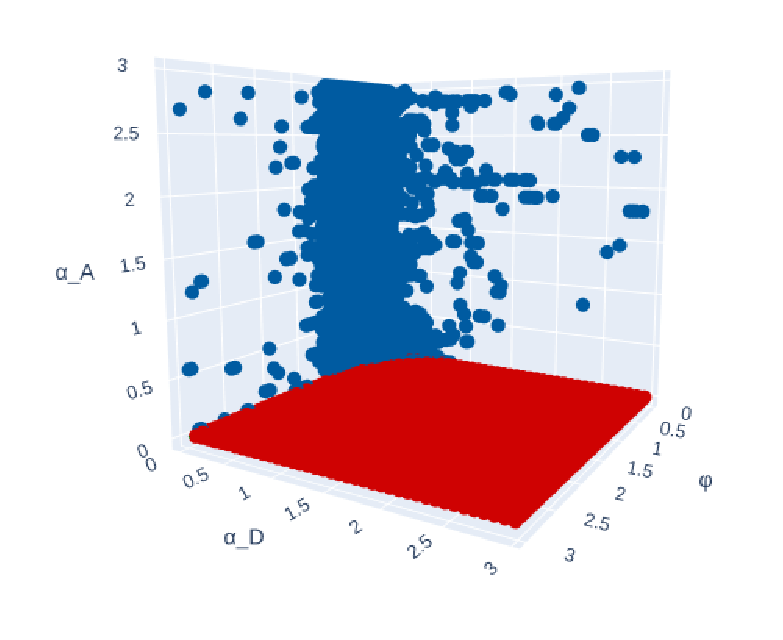
\includegraphics[width=0.9\linewidth]{figs/approx_surface_decision_space.eps}
    \caption{Decision space for FlipIt with IE with approximated BRDVs for the defender plotted in blue and those for the attacker in red.}
    \label{fig:approx_surface}
\end{figure}

Regardless of the shape of these geometric figures, since by definition each PSNE is a state in which all players play a BRDV simultaneously, we can think of the PSNEs as the intersections of the figures for all players.
This concept has been explicitly used for single-objective players in \cite{dijk2013flipit} and implicitly in the EA implementation by \cite{sherfield2018flipthem}, but to the best of our knowledge, it has not been generalized to multi-objective players or multi-player games until now.


\subsection{Numerical Approximation Procedure}

The problem with the idealized procedure is that it is not feasible to run infinite independent multi-objective optimizations on digital computers.
Moreover, each optimization is also not perfectly continuous, as even ``real'' variables are represented with a finite number of bits in a computer; although for all practical purposes we can consider them ``real'' valued.

To address these limitations while still confirming the theoretical foundations of the idealized procedure, we propose a numerical procedure that discretizes the OSPs for each player, then approximates the BRDVs for each OSP using a regular multi-objective evolutionary algorithm.
This approach avoids game-theory-specific fitness functions (see \cite{leite2024cec}, \cite{lung2008computing}, \cite{lung2020pareto}), adopting a Pareto-Front approach that should appear more intuitive to researchers in the field of computational optimization.
The PSNEs are then computed as the points from each player that are within a small arbitrary distance $\epsilon$ from a point for every other player (i.e., the intersection of the approximated BRDVs).

The procedure overview is shown in Algorithm \ref{alg:approximation}.

\begin{algorithm}[h]
    \SetAlgoLined
    
    \KwIn{\\
        \begin{tabular}{ll}
            \texttt{players} & Player data\\
            \texttt{bounds} & Decision variable bounds\\
            \texttt{n\_dims} & Grid divisions per decision\\
            \texttt{n\_gens} & Number of generations\\
            \texttt{n\_nest\_gens} & Nested generations per gen.\\
            \texttt{$\epsilon$} & Intersection threshold\\
        \end{tabular}
    }

    \For{\texttt{p} \textbf{in} \texttt{players}}{
        \texttt{p.osps} $\leftarrow$ \texttt{get\_osps}(\texttt{p}, \texttt{bounds}, \texttt{n\_dims})\;
        \For{\texttt{osp} \textbf{in} \texttt{p.osps}}{
            \texttt{p.eas.add}(new EA for \texttt{p} and \texttt{osp})\;
        }
    }

    \For{\texttt{g} \textbf{in} \texttt{1} \textbf{to} \texttt{n\_gens}}{
        
        \For{\texttt{p} \textbf{in} \texttt{players}}{
            \For{\texttt{osp} \textbf{in} \texttt{p.osps}}{
                \texttt{ea} $\leftarrow$ EA for \texttt{osp} in \texttt{p.eas}\;
                \texttt{ea.run}(\texttt{n\_nest\_gens})\;
                \tcp{Evaluates w/ \texttt{p.fitness\_fn}}
            }
        }
        
        \texttt{psnes} $\leftarrow$ \texttt{intersection}(\texttt{players}, \texttt{$\epsilon$})\;
        \texttt{fits} $\leftarrow$ fitness \textbf{for} \texttt{psne} \textbf{in} \texttt{psnes}\;
    }

    \KwOut{\\
        \begin{tabular}{ll}
            \texttt{psnes} & Approximated solutions\\
            \texttt{fitnesses} & Fitness values for approxs.\\
        \end{tabular}
    }
    \caption{Numerical approximation of PSNEs}
    \label{alg:approximation}
\end{algorithm}



\section{Experimental Setup}
\label{methodology}

The game model used for the experiments was FlipIt with IE and Periodic Strategies (PS) \cite{leite2024cec}, with $φ_0=5$, $k_0=1.0$, $k_1=1.5$, and $c=0.2$.
The decision space was discretized into a 40x40x160 grid, with minimum and maximum bounds of 0.01 and 3.00, respectively, for the defender's $\phi$, and 0.005 and 3.00, respectively, for the defender's $\alpha_0$ and the attacker's $\alpha_1$.
Game results were evaluated algebraically through the payoff functions for each player \cite{leite2024cec}.

NSGA-II was chosen as the multi-objective evolutionary algorithm for each BRDV approximation, even though the BRDVs for the attacker are actually single-objective problems.
This was done to keep the experimental code short and simple, even though a single-objective algorithm could (and arguably should) be specially allocated for single-objective players.
The algorithm was executed for 400 generations, with each nested GA running 100 generations each time.


\section{Results and Discussion}
\label{results}


The experiment results are shown in Fig.~\ref{fig:approx_psne}.
The figure displays the approximated PSNEs as dots, with defender decision variables on the horizontal axes and the attacker's $\alpha_1$ on the vertical axis.
The analytically determined (ideal) PSNE curve is shown as a continuous line, providing a reference for assessing the numerical results.
Fig.~\ref{fig:approx_fitness} shows the fitness values for each approximated PSNE.

\begin{figure}[h]
    \centering
    % Converted with: pdftops -eps figs/approx_psne_decision_space.pdf
    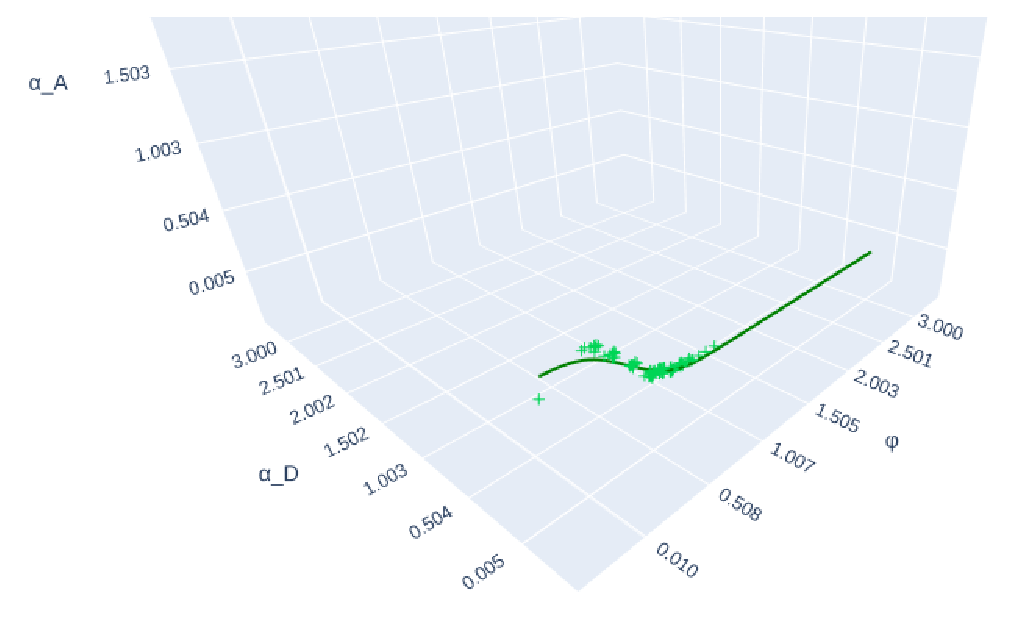
\includegraphics[width=0.9\linewidth]{figs/approx_psne_decision_space.eps}
    \caption{Approximated PSNEs for FlipIt with IE and PS shown as dots; the continuous line represents the ideal PSNE curve.}
    \label{fig:approx_psne}
\end{figure}

\begin{figure}[h]
    \centering
    % Converted with: pdftops -eps figs/approx_psne_objective_space.pdf
    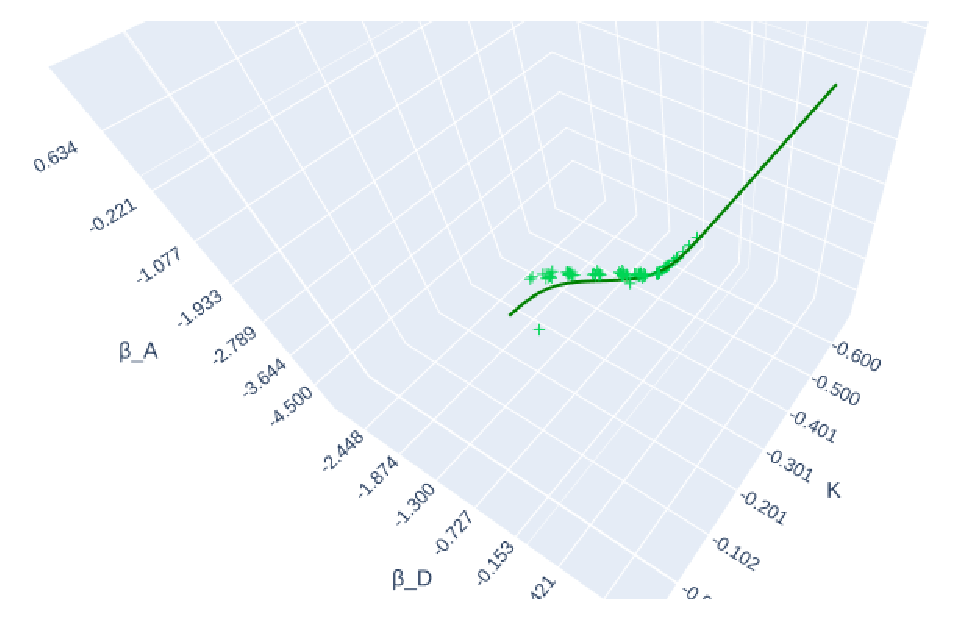
\includegraphics[width=0.9\linewidth]{figs/approx_psne_objective_space.eps}
    \caption{Fitness of the solutions found vs. the ideal fitness curve.}
    \label{fig:approx_fitness}
\end{figure}

As can be seen, the approximations closely follow the ideal curve, with very few outliers (in the current run, only one is present).
The average distance of the approximations to the ideal curve for this run is 0.0381, with a standard deviation of 0.0255.
This rivals the results obtained in \cite{leite2024cec}.

The number of estimations (77), while far from the previously obtained number and even further from the ideal (infinite), is sufficient to provide a good visual representation of the PSNE curve.
These results suggest that the proposed method is effective in numerically approximating PSNEs for continuous games of simultaneous decision, providing valuable insights into the game's equilibrium tendencies even in the absence of analytical solutions.

\section{Conclusions and Future Work}
\label{conclusions}

This paper presented both an idealized procedure and a numerical approximation procedure for solving continuous games of simultaneous decision that can be easily adapted to any number of players, objectives, and solutions.
The numerical approximation procedure was shown to be effective in finding a finite number of PSNEs for FlipIt with IE, a game with one single-objective player, one multi-objective player, and three continuous decision variables in total.

The approximations found exhibited a good distribution and a low noise level despite the reduced number of actual estimations.
With this method, the analyst can obtain a visual representation of the game's equilibrium tendencies, even for cases where analytical solutions are unavailable.
The proposed method offers an approach that may be intuitive for researchers in the field of computational optimization, as the EAs are not modified with game-theory-based fitness functions.
It should also be intuitive for researchers in the field of game theory, as the convergence criterion essentially generalizes the game-theoretical concept of ``all players playing best responses simultaneously''.
We hope that the framework provided here can guide the development of new, more efficient methods to solve game-theoretical models of simultaneous decision and continuous decision spaces.

As future work, we plan to increase the method's computational efficiency by enhancing the intersection-computing algorithm, allowing for a finer grid, faster convergence, and, hopefully, a larger and less noisy set of estimations.

\bibliographystyle{plain}
\bibliography{symposium}

%------------------------------------------------------------------------------
\end{document}
